
Cilk was originally developed in the 1990’s at Massachusetts Institute of Technology. It was
later productized and commercialized by a spinoff company, Cilk Arts. During the 2000’s Cilk
Arts targeted the high performance and highly parallel multi-core computer market, which were emerging as consumer commodity products at the time. Intel acquired Cilk Arts in 2009 and codeveloped Cilk’s enhancements with its hardware. The current version of Cilk being investigated in this report is Cilk Plus. This is Intel’s development branch of Cilk that is tuned to Intel’s C/C++ Compiler; however, it is also available in GCC versions 4.9 and above. In this
paper, the terms Cilk and Cilk Plus will be used interchangeably, despite their semantic
differences.

Cilk is a faithful extension of C/C++. One of the key principles of Cilk is that the
programmer should be responsible for exposing the parallelism of the algorithm and should
identify those elements that lend themselves to be parallelized. The scheduling and execution
model should be left to the processor hardware. This philosophy is important in the sense that the degree of parallelism is ultimately determined by the hardware and system resources. Such an approach to parallelism is ideal when trying to measure and calculate the theoretical growth of certain algorithms that lend themselves to be parallelized. The Cilk framework can leverage the hardware capabilities of the system by having the programmer expose as much parallelism in the algorithms using Cilk keywords.


\subsection{How Cilk Works}
The Cilk scheduler, which is what Cilk uses to divide work during execution among multiple processors, is based on the concept of “work-stealing”. Specifically, Cilk uses greedy work-stealing algorithms to assign specific function tasks to available cores. The programmer exposes those functions that are parallelizable using a variety of keywords. The main two are the “spawn” and “sync” keywords; however, Cilk has expanded its constructs to include the \texttt{cilk\_for} construct.

Cilk follows certain rules regarding spawned functions’ parent-child relationships. For example, a child cannot view a sibling’s data, only the parent’s. However, when the child finishes executing or is idle a processor will try to “steal” work from a sibling. This is achieved with “cactus stacks”. In these kinds of stacks, the activation frames of Cilk procedures are pushed onto the stack and idle processors try to take the most recently pushed work available.

The programmer will signal to the compiler that a function is a Cilk function with the keyword cilk in the function declaration. In the body of the function the keyword “spawn” is used to signal that a parallelizable procedure is to be used and that a parent-child relationship exists. The parent will not be able to return until all spawned children have “sync[ed]”. If this parallelism is done in a recursive fashion, deep parent-child functions will exist giving it the “cactus” appearance.

\begin{figure}
\center
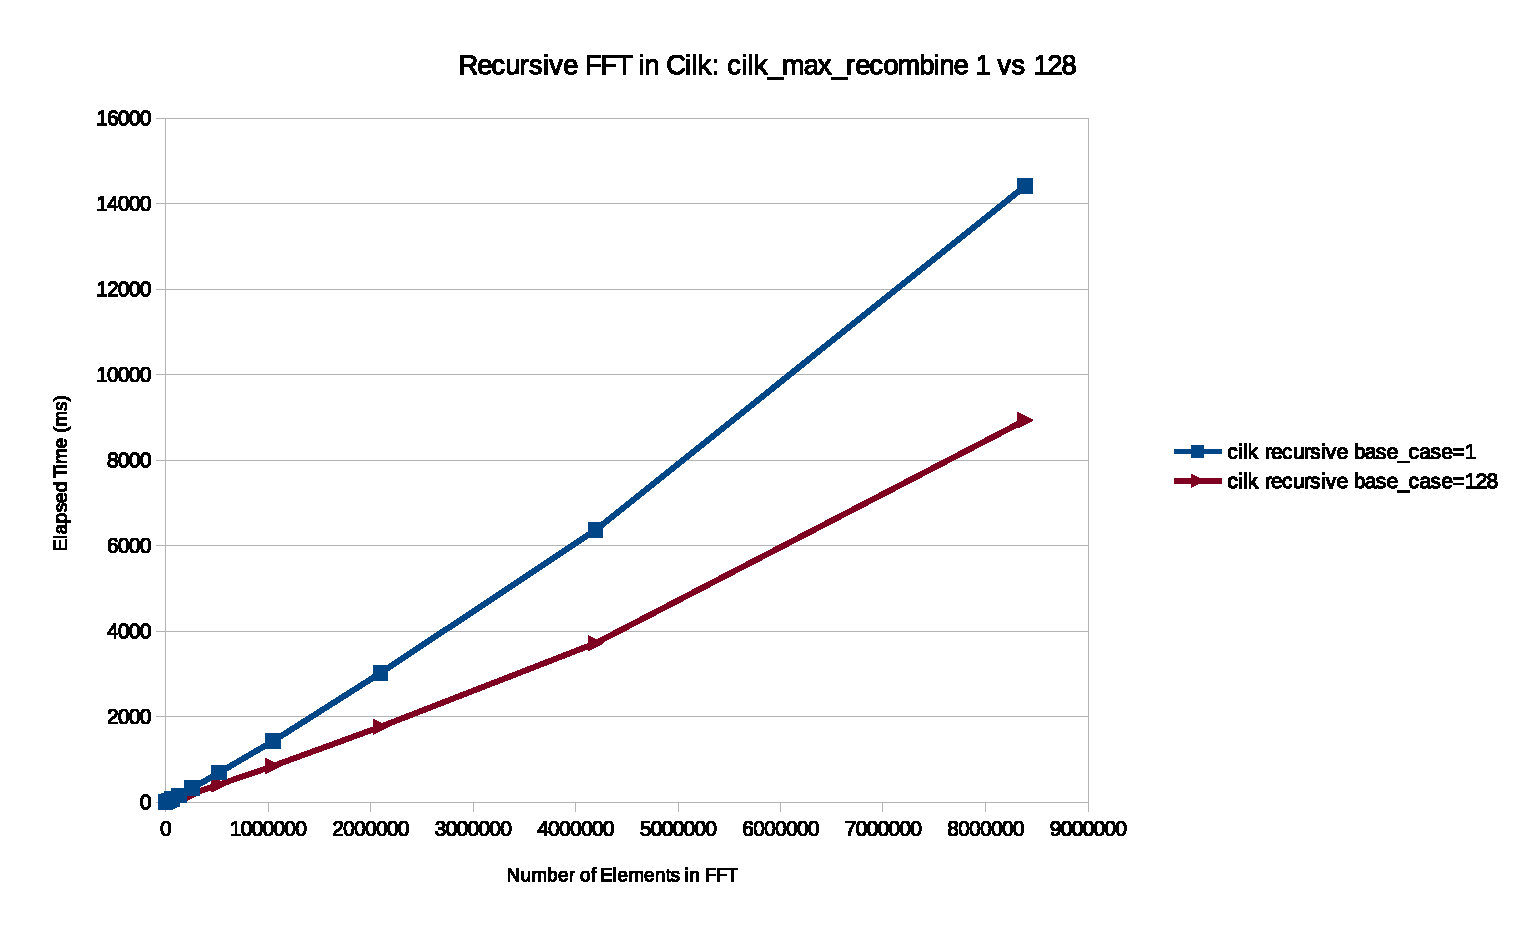
\includegraphics[scale=0.8]{img/cilk_max_recombine.eps}
\caption{Graph comparing the two cilk recursive runs with values of \texttt{cilk\_max\_recombine}=1,128} 
\label{cilk_max_recombine}
\end{figure}

\begin{figure}
\center
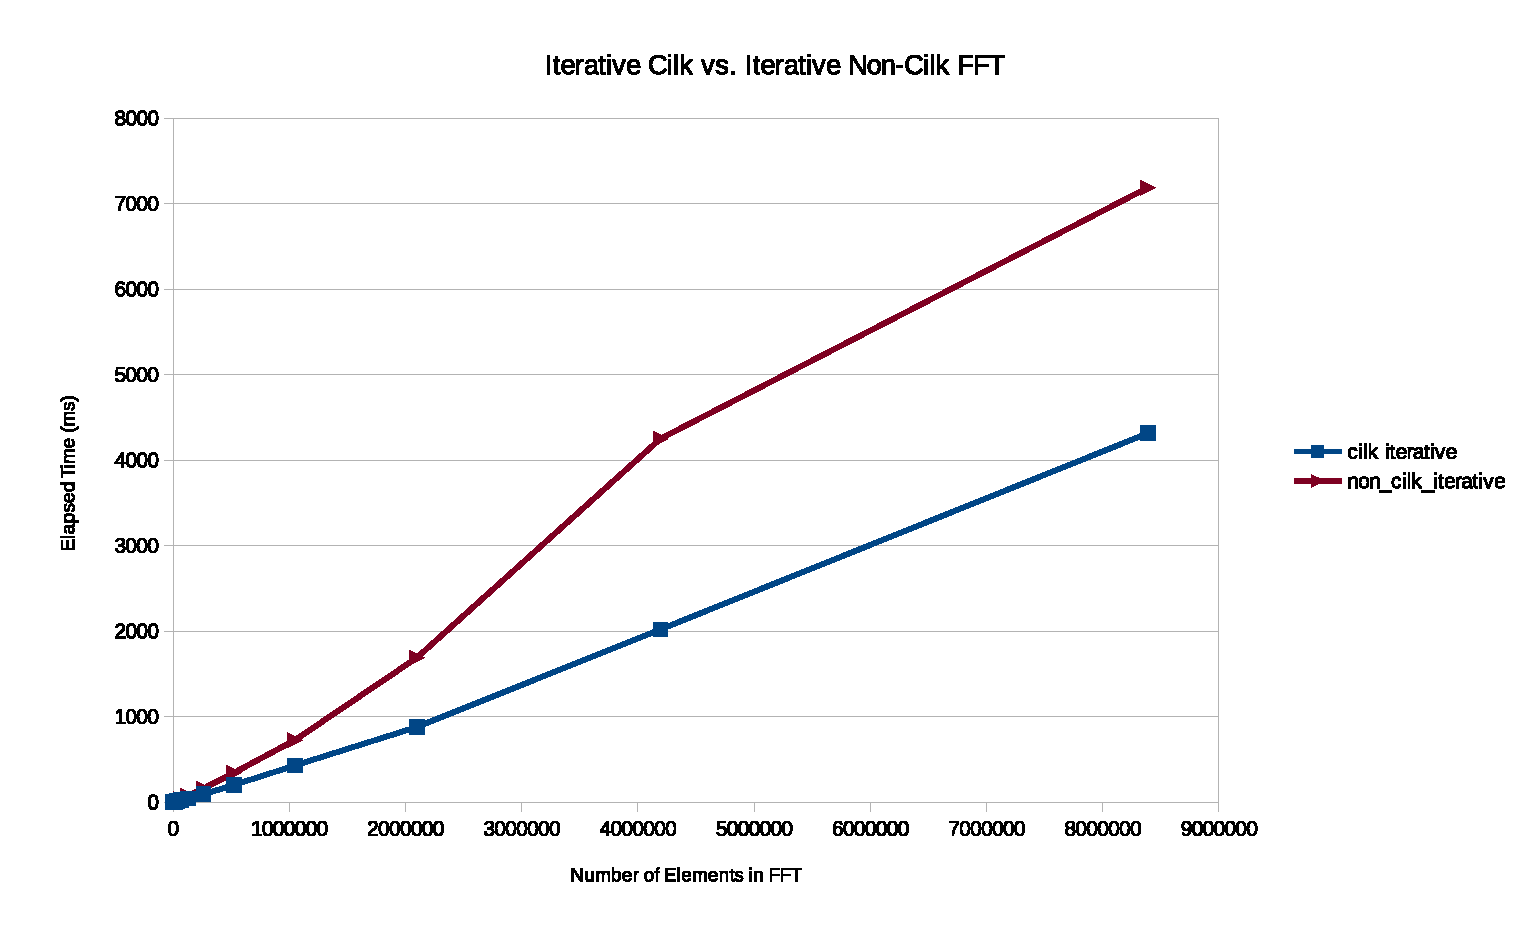
\includegraphics[scale=0.8]{img/iterative_fft.eps}
\caption{Graph comparing the performance of the iterative cilk and non-cilk (C++) FFT algorithms} 
\label{iterative_fft}
\end{figure}


\begin{landscape}
\thispagestyle{empty}
\begin{figure}
\centering
        \begin{subfigure}[b]{0.65\textwidth}
            \center
            \includegraphics[width=\textwidth]{img/fft_iter_cilk.png}
            \caption{Heap memory usage of iterative cilk algorithm}
            \label{fig:heap_iter_cilk}
        \end{subfigure}%
        \begin{subfigure}[b]{0.65\textwidth}
            \center
            \includegraphics[width=\textwidth]{img/fft_iter_cpp.png}
            \caption{Heap memory usage of iterative C++ algorithm}
            \label{fig:heap_iter_cpp}
        \end{subfigure}%
        \vskip\baselineskip
        \begin{subfigure}[b]{0.65\textwidth}
            \center
            \includegraphics[width=\textwidth]{img/fft_rec_cilk.png}
            \caption{Heap memory usage of recursive cilk algorithm}
            \label{fig:heap_rec_cilk}
        \end{subfigure}%
        \begin{subfigure}[b]{0.65\textwidth}
            \center
            \includegraphics[width=\textwidth]{img/fft_rec_cpp.png}
            \caption{Heap memory usage of recursive C++ algorithm}
            \label{fig:heap_rec_cpp}
        \end{subfigure}
        \caption{Valgrind's masiff Heap tracer for cilk vs C++}\label{fig:masiff}
\end{figure}
\end{landscape}